% =============================================================
% OPTION B: Minimal Surgical Edits — Remove Duplication and Add Bridges
% =============================================================
% Drop-in replacement for the Objective 7 section in chapter3.tex
% (replaces lines 1354–1517)
% =============================================================

\section{Objective 7: Task Category Level Task-Modality Qualification Mapping}
\label{sec:ch3_obj7_category_taskmodality}

Objective 7 converts validated measurement instruments (Objective~5) and resource accounting (Objective~6) into guidance given comparable MCQ and OSQ measurements, which evaluation modality is most defensible for each systems engineering task category. Whereas Objective~5 answers "can we trust these measurements?" and Objective~6 answers "what do they cost?", Objective~7 answers "what modality should be used, by category, under the observed evidence patterns?"

This objective produces an auditable mapping from INCOSE 15288 aligned task categories to modality recommendations (e.g., MCQ-sufficient, OSQ-preferred, dual-modality required). The mapping is generated by (i) decomposing multi-label category assignments to compute per-category performance under each modality, (ii) quantifying per-category modality advantage via an MCQ--OSQ delta analysis, and (iii) applying a predefined decision tree that converts delta magnitude, absolute performance, and cross-model variability into a qualification recommendation.


% ---------------------------------------------------------
\subsection{Category Decomposition and Alignment}
\label{subsec:ch3_obj7_category_decomposition}

Each SysEngBench item includes one or more INCOSE-aligned category labels. Objective~7 uses these labels to compute performance \emph{per category}.

Some questions are tagged with multiple categories. To avoid forcing a single label, the data is "exploded": a question with $k$ labels contributes once to each of its $k$ categories. The question ID is retained so any category-level statistic can be traced back to the underlying items.

Two levels of granularity are analyzed:

\begin{enumerate}[nosep]
    \item Leaf-level categories ($\approx$20): the most specific INCOSE process or topic area (e.g., \textit{Risk and Opportunity Management Process}, \textit{Modeling Language SysML v1.x}).
    \item \Top-level groups ($\approx$6): the second level of the hierarchy (e.g., \textit{Technical Processes}, \textit{Specialty Engineering Activities}, \textit{Cross-Cutting Systems Engineering Methods}).
\end{enumerate}

Analyzing at both levels tests whether modality differences are driven by specific leaf categories or are systematic properties of entire process families.

\begin{table}[htbp]
\centering
\caption{SysEngBench INCOSE Category Roll-Up Mapping}
\label{tab:sysengbench_category_rollup}
\small
\renewcommand{\arraystretch}{1.15}
\begin{tabular}{p{4.2cm} p{10.2cm}}
\toprule
\textbf{Top-level category} & \textbf{Leaf-level categories within top-level} \\
\midrule
Cross-Cutting Systems Engineering Methods &
$\bullet$ Model-Based Systems Engineering / Modeling Frameworks and Methods \newline
$\bullet$ Model-Based Systems Engineering / Modeling Language SysML v1.x \newline
$\bullet$ Modeling and Simulation \\
\midrule
Lifecycle Stages &
$\bullet$ Defense Acquisition Life Cycle / Lifecycle Phases \newline
$\bullet$ Defense Acquisition Life Cycle / Milestones and Reviews \newline
$\bullet$ Generic Life Cycle Stages \\
\midrule
Specialty Engineering Activities &
$\bullet$ Cost Modeling \newline
$\bullet$ Electromagnetic Compatibility \newline
$\bullet$ Reliability, Availability, and Maintainability \newline
$\bullet$ Supportability, Producibility and Disposability \newline
$\bullet$ System Safety Engineering \newline
$\bullet$ Usability and Human Systems Integration \\
\midrule
Systems Engineering Overview &
$\bullet$ Application and Value of Systems Engineering \newline
$\bullet$ System Concepts and Structures \newline
$\bullet$ Systems Science and Thinking \\
\midrule
Technical Management Processes &
$\bullet$ Configuration and Information Management \newline
$\bullet$ Decision Management, Analysis of Alternatives, and Tradespace Analysis \newline
$\bullet$ Risk and Opportunity Management Process \\
\midrule
Technical Processes &
$\bullet$ Architecture Definition Process \newline
$\bullet$ Identifying Stakeholder Needs and Generating Requirements \\
\bottomrule
\end{tabular}
\end{table}

Category-level estimates are only used for modality recommendations when the category has at least $n_{\min}$ contributing questions (after exploding multi-label items). Categories below this threshold are still shown descriptively (e.g., counts/heatmaps) but are excluded from prescriptive guidance.

Let $\mathcal{I}(c)$ be the set of questions assigned to category $c$ (after exploding multi-label items). Accuracy for modality $q$ is:
\[
\text{Acc}_{q,c}=\frac{1}{|\mathcal{I}(c)|}\sum_{i\in \mathcal{I}(c)} \mathbb{I}[\text{correct}(i,q)].
\]

These per-category accuracy estimates provide the inputs for the performance comparison and modality advantage analysis that follow.


% ---------------------------------------------------------
\subsection{Category-Level MCQ and OSQ Performance}
\label{subsec:ch3_obj7_performance}

Before quantifying modality advantage, per-category performance under each modality is examined independently. For each (model, category) pair, two performance metrics are computed:

\begin{itemize}[nosep]
    \item \textbf{MCQ accuracy}: the proportion of correct responses across all position variants for questions in that category ($\overline{\text{Acc}}_{\text{MCQ}}$, range 0--1).
    \item \textbf{OSQ mean score}: the average rubric-based percentage score across all judge evaluations for questions in that category ($\overline{S}_{\text{OSQ}} / 100$, normalized to 0--1).
\end{itemize}

Results are presented as model $\times$ category heatmaps for each modality, with models sorted by overall MCQ accuracy (descending) and categories sorted alphabetically. This consistent ordering across MCQ and OSQ heatmaps supports direct visual comparison.

A category-level scatter plot analogous to the model-level MCQ vs.\ OSQ scatter (Objective~5, Section~\ref{subsec:ch3_obj5_modality_comparison}) is constructed for each granularity level: one point per category, with coordinates $(\overline{\text{Acc}}_{\text{MCQ}},\; \overline{S}_{\text{OSQ}})$ averaged across all models. A perfect-agreement line ($y = x$) and linear regression are overlaid to visualize systematic modality divergence by domain area.


% ---------------------------------------------------------
\subsection{Modality Advantage Quantification}
\label{subsec:ch3_obj7_delta}

With per-category MCQ and OSQ performance established, the modality advantage for each category can now be quantified. The MCQ--OSQ delta captures the direction and magnitude of modality advantage for each (model, category) pair:

\[
\Delta_{m,c} \;=\; \overline{\text{Acc}}_{\text{MCQ},m,c} \;-\; \frac{\overline{S}_{\text{OSQ},m,c}}{100}
\]

where $m$ indexes models and $c$ indexes categories. Positive values indicate MCQ advantage (recognition exceeds generation); negative values indicate OSQ advantage.

Results are reported as delta heatmap tables: a model $\times$ category matrix of $\Delta_{m,c}$ values with marginal summary statistics. The final column reports per-model mean and median $\Delta$ (across categories); the final row reports per-category mean and median $\Delta$ (across models). This structure, analogous to a joint probability table, enables simultaneous reading of model-level and category-level modality tendencies.

As a design prior, MCQ (selected-response) performance is treated as a lower-effort evidence type than OSQ (constructed-response) because MCQs provide answer cues and permit partial-knowledge strategies (e.g., recognition and elimination), whereas OSQs require generating and justifying an answer without options. This distinction is widely discussed in assessment and measurement guidance and is a primary motivation for using constructed-response formats when explanation, reasoning, or argumentation quality is part of the intended inference \cite{livingston_ConstructedResponseTestQuestionsWhy_2009, AmEdAssoc_StandardsForEducationalTesting_2014}. Therefore, it is pre-specified that some task families may show materially different apparent competence under MCQ versus OSQ, and large modality gaps in either direction are treated as a form of modality sensitivity, triggering dual-modality evidence rather than a single-modality prescription.

To translate delta magnitudes into actionable guidance, each category is classified into one of four modality recommendations based on the cross-model mean delta ($\overline{\Delta}_c$) and the mean MCQ accuracy for that category ($\overline{\text{Acc}}_{\text{MCQ},c}$):

\begin{table}[htbp]
\centering
\caption{Predefined category-level qualification modality classification criteria.}
\label{tab:obj7_classification}
\resizebox{\linewidth}{!}{%
\begin{tabular}{p{3.6cm} p{4.2cm} p{3.2cm} p{6.2cm}}
\toprule
\textbf{Classification} & \textbf{Mean delta $|\overline{\Delta}_c|$} & \textbf{Mean MCQ Acc.} & \textbf{Interpretation and Guidance} \\
\midrule
MCQ-sufficient &
$|\overline{\Delta}_c| < 0.05$ &
$\overline{\text{Acc}}_{\text{MCQ},c} \geq 0.85$ &
Modalities are effectively equivalent and MCQ accuracy is already high. MCQ captures competence adequately; OSQ is optional and can be reserved for higher-risk follow-up. \\
\addlinespace
Dual-modality recommended &
$0.05 \leq |\overline{\Delta}_c| < 0.15$ &
Any &
Meaningful modality gap exists regardless of direction. Use MCQ for breadth and OSQ for confirmation on moderate/high-risk uses; investigate whether MCQ guess-ability or OSQ scoring strictness contributes to the gap. \\
\addlinespace
Dual-modality required &
$|\overline{\Delta}_c| \geq 0.15$ &
Any &
Large modality divergence in either direction. Results are modality-sensitive; require both modalities for qualification evidence and investigate the source of the discrepancy (e.g., MCQ inflation via guessing or OSQ construct differences). \\
\addlinespace
Insufficient coverage &
Any &
$< 30$ samples in category &
Too few observations for reliable classification. Report descriptive statistics only; do not assign modality recommendation. \\
\bottomrule
\end{tabular}
}
\noindent\textit{Note.} Read each row as an AND rule: a category must meet both the delta condition and the MCQ accuracy condition unless the column says \emph{Any}. The \emph{Insufficient coverage} rule is checked first and overrides the others. All delta thresholds use absolute values, making the classification symmetric with respect to modality direction.
\end{table}


Figure~\ref{fig:cross-mod-class-regions} provides a geometric interpretation of the classification criteria defined in Table~\ref{tab:obj7_classification}. Each point in the plot represents a hypothetical category with a given mean MCQ accuracy ($x$-axis) and mean OSQ accuracy ($y$-axis). The diagonal line $y = x$ marks perfect modality agreement ($\Delta = 0$). The green region in the upper-right corner identifies categories classified as \emph{MCQ-sufficient}, requiring both high MCQ accuracy ($\geq 85\%$) and near-diagonal placement ($|\Delta| < 5$ percentage points). The amber bands flanking the diagonal correspond to \emph{dual-modality recommended} categories ($5 \leq |\Delta| < 15$), while the red regions beyond the outer boundaries denote \emph{dual-modality required} categories ($|\Delta| \geq 15$). Because all thresholds are defined on the absolute delta, the regions are symmetric about the diagonal where a large MCQ advantage and a large OSQ advantage of equal magnitude receive the same classification.

\begin{figure}[htbp]
    \centering
    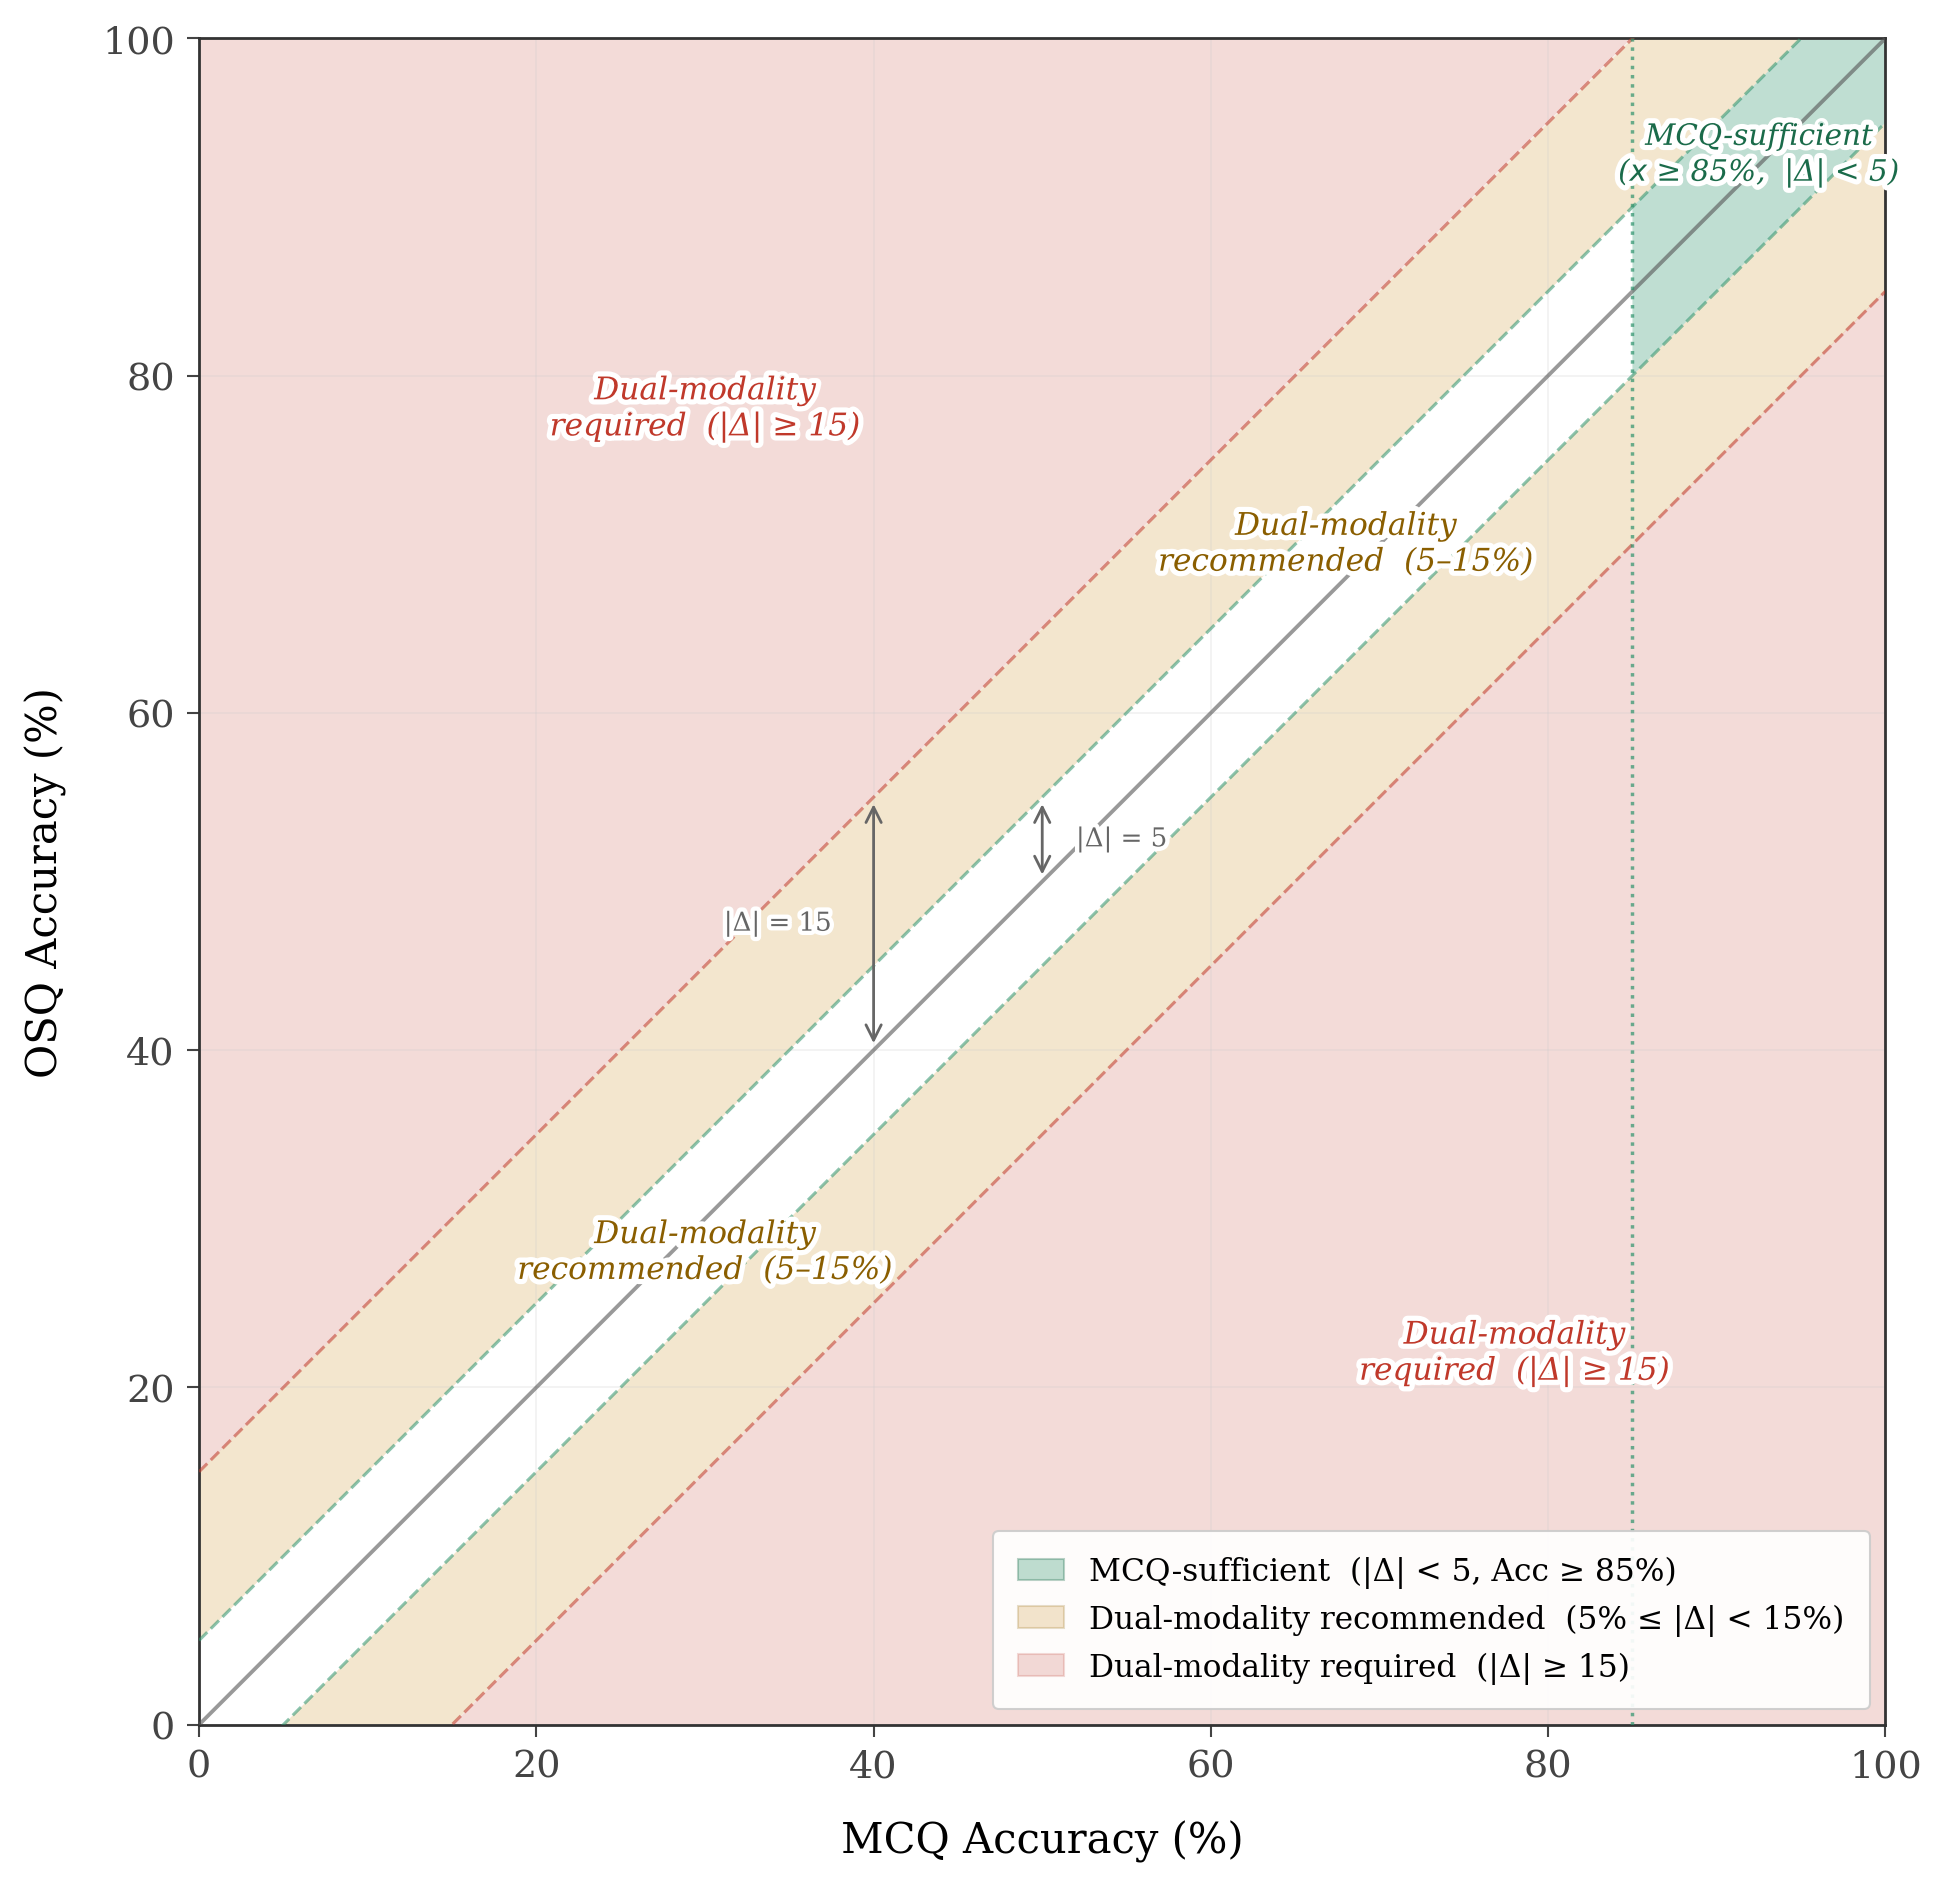
\includegraphics[width=0.8\textwidth]{figs/ch3/obj7_classification_regions.png}
    \caption{Cross-Modality Classification Regions}
    \label{fig:cross-mod-class-regions}
\end{figure}

The thresholds are applied independently at both granularity levels, including leaf categories and top-level groups. The classification is intended as a structured starting point for deployment decisions; organizations should adjust thresholds based on their risk tolerance and domain-specific requirements. This expectation is tested and quantified empirically in Chapter~4 using the category-level MCQ/OSQ accuracy and delta analyses.
